\section{Auswertung}
\label{sec:Auswertung}
Es wurden aus \autoref{abb:Entladung} die Werte in \autoref{tab:DatenEntladung} entnommen und nach Gleichung \eqref{RelQ} folgt 
für die lineare Regression:
\begin{equation}
  \label{eqn:linRegress}
    \ln\left(\frac{U_c}{U_0}\right)=-\frac{1}{RC}\cdot t + b.
\end{equation}
Woraus die Zeitkonstante $RC$ bestimmt wird.

\begin{figure}
  \centering
  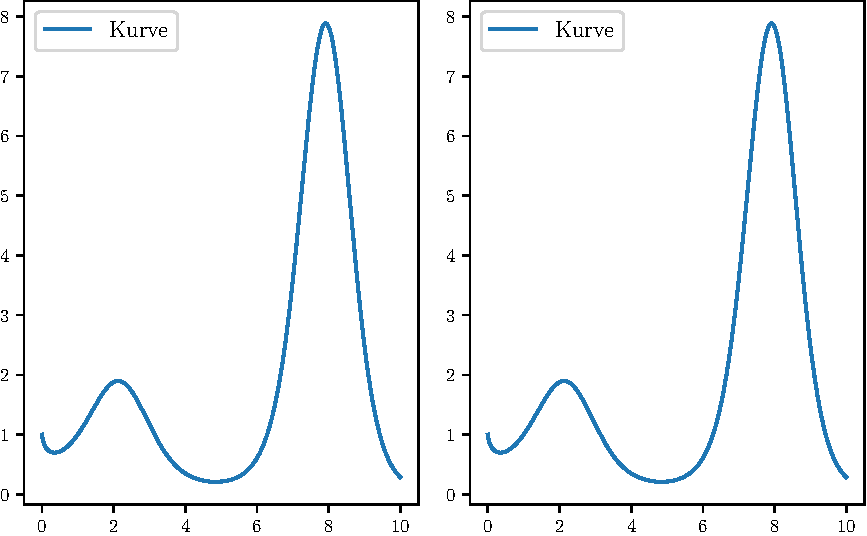
\includegraphics{plot.pdf}
  \caption{Lineare Regression nach \eqref{eqn:linRegress} und Messdaten aus \autoref{tab:DatenEntladung} zur Bestimmung der Zeitkonstante RC über den Entladungsprozesses des Kondensators.}
  \label{fig:plot}
\end{figure}

Es ergibt sich aus der linearen Regression in \autoref{fig:plot}:
\begin{align*}
  RC &= (0.39001\pm 0.00056)\unit{\milli\second}\\
  b &= 0.030872\pm 0.021421.\\
\end{align*}
%(-2564.035208002769, 37.56001783858995, 0.03087285853896417, 0.02142147040602549)
Anschließend wurde die Zeitkonstante $RC$ mit den Wertepaaren der Relativamplitude $\frac{U_c}{U_0}$ und der Generatorfrequenz $f$
aus \autoref{tab:DatenB} mithilfe der folgende Ausgleichsrechnung bestimmt:
\begin{equation}
  \label{eqn:Ausgleichsrechnung1}
  \frac{U_c}{U_0} = e^{(-a\cdot f + b)}.
\end{equation}
Wobei bei dieser Ausgleichsrechnung die Zeitkonstante $RC = a$ ist.
\begin{figure}
  \centering
  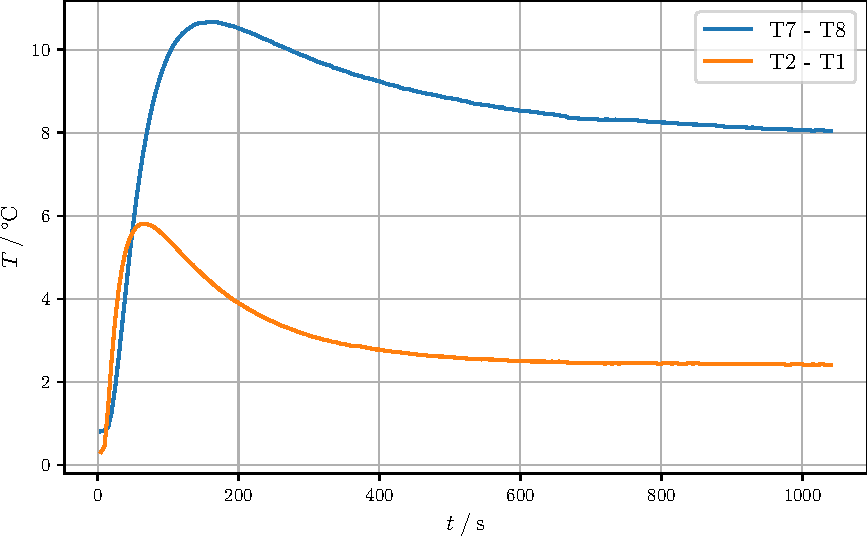
\includegraphics{plot2.pdf}
  \caption{Hier sind die Wertepaare aus \autoref{tab:DatenB} die Ausgleichsrechnung nach \eqref{eqn:Ausgleichsrechnung1} und die Originalfunktion nach \eqref{eqn:bezAU} mit dem berechneten $RC$ in einem halblogarithmischen Diagramm aufgetragen.}
  \label{fig:plot2}
\end{figure}

Es ergeben sich die Parameter a und b der Ausgleichsrechnung zu:
\begin{align*}
  a &= (2.6401\pm 0.2442) \unit{\milli\second} = RC\\
  b &= 0.99545\pm 0.06030\\
\end{align*}

Die dritte Methode, die Zeitkonstante $RC$ zu bestimmen, basiert auf einer Ausgleichsrechung zu den Wertepaaren der Phasenverschiebung $\varphi$ 
und der Generatorfrequenz $f$ aus \autoref{tab:DatenC}.
Die Ausgleichsrechnung ergibt sich in diesem Fall nach \eqref{PhiArctan} zu:
\begin{equation}
  \label{eqn:Ausgleichsrechnung2}
  \symup{\varphi} = a\cdot\arctan(b\cdot t).
\end{equation}
Wobei hier die Zeitkonstante $RC = b$ ist.
\begin{figure}
  \centering
  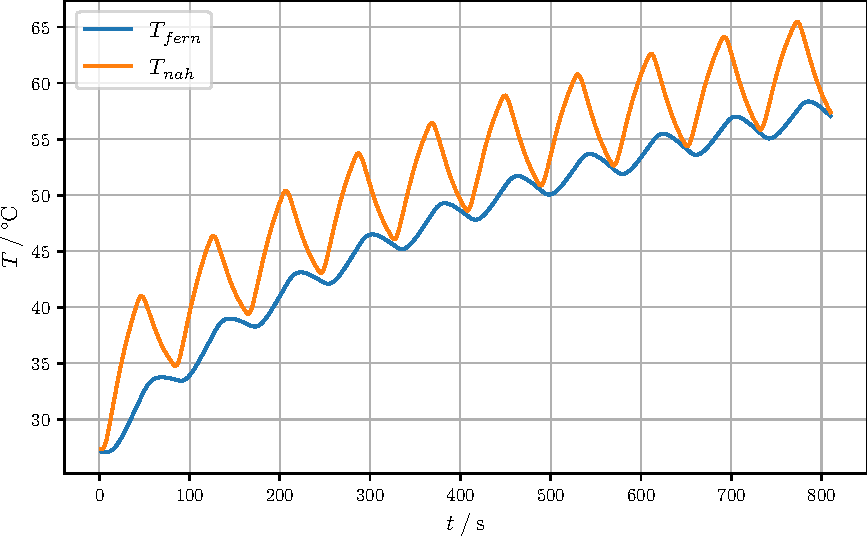
\includegraphics{plot3.pdf}
  \caption{Hier sind die Wertepaare aus \autoref{tab:DatenC}, die Ausgleichsrechnung nach \eqref{eqn:Ausgleichsrechnung2} und die Originalfunktion nach \eqref{PhiArctan} mit eingesetztem $RC$ in einem halblogarithmischem Diagramm aufgetragen.}
  \label{fig:plot3}
\end{figure}
Bei dieser Ausgleichsrechnung ergeben sich die Parameter a und b zu:
\begin{align*}
  a &=0.9862\pm 0.0464 \\
  b &=(6.9641\pm 2.0824) \unit{\milli\second} = RC \\
\end{align*}

Die Abhängigkeit der Relativamplitude $\frac{U_c}{U_0}$ von der Phase $\varphi$ ergibt sich zu:
\begin{equation*}
  \frac{U_c}{U_0} = \cos\left(\varphi\right).
\end{equation*}

\begin{figure}
  \centering
  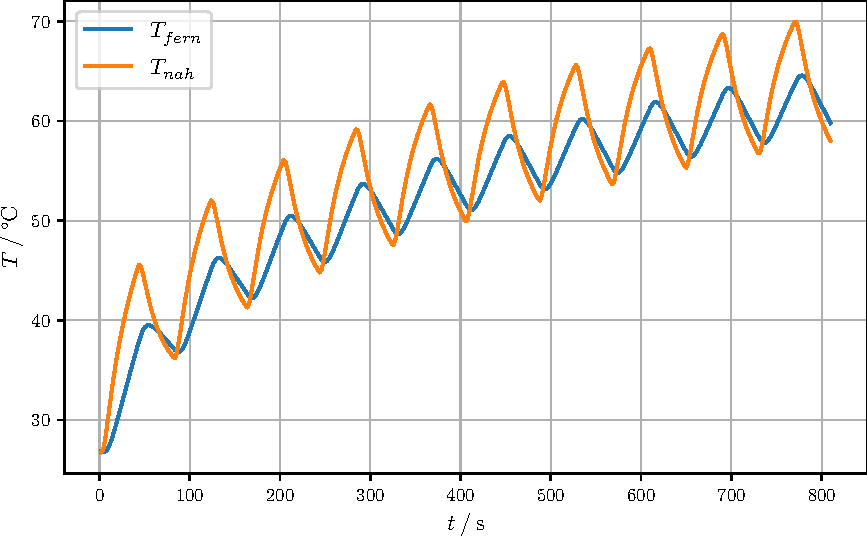
\includegraphics{plot4.pdf}
  \caption{Hier wurde die erwähnte Abhängigkeit der Relativamplitude von der Phase, sowie einige Wertepaare aus \autoref{tab:DatenD} in ein Polardiagramm eingetragen.}
  \label{fig:plot4}
\end{figure}

\begin{figure}
  
  \centering
  \textbf{Integration verschiedener Generatorspannungen bei einer Frequenz $\symbf{f = 4726\unit{\hertz}}$}\par\medskip
  \begin{subfigure}{0.48\textwidth}
    \centering
    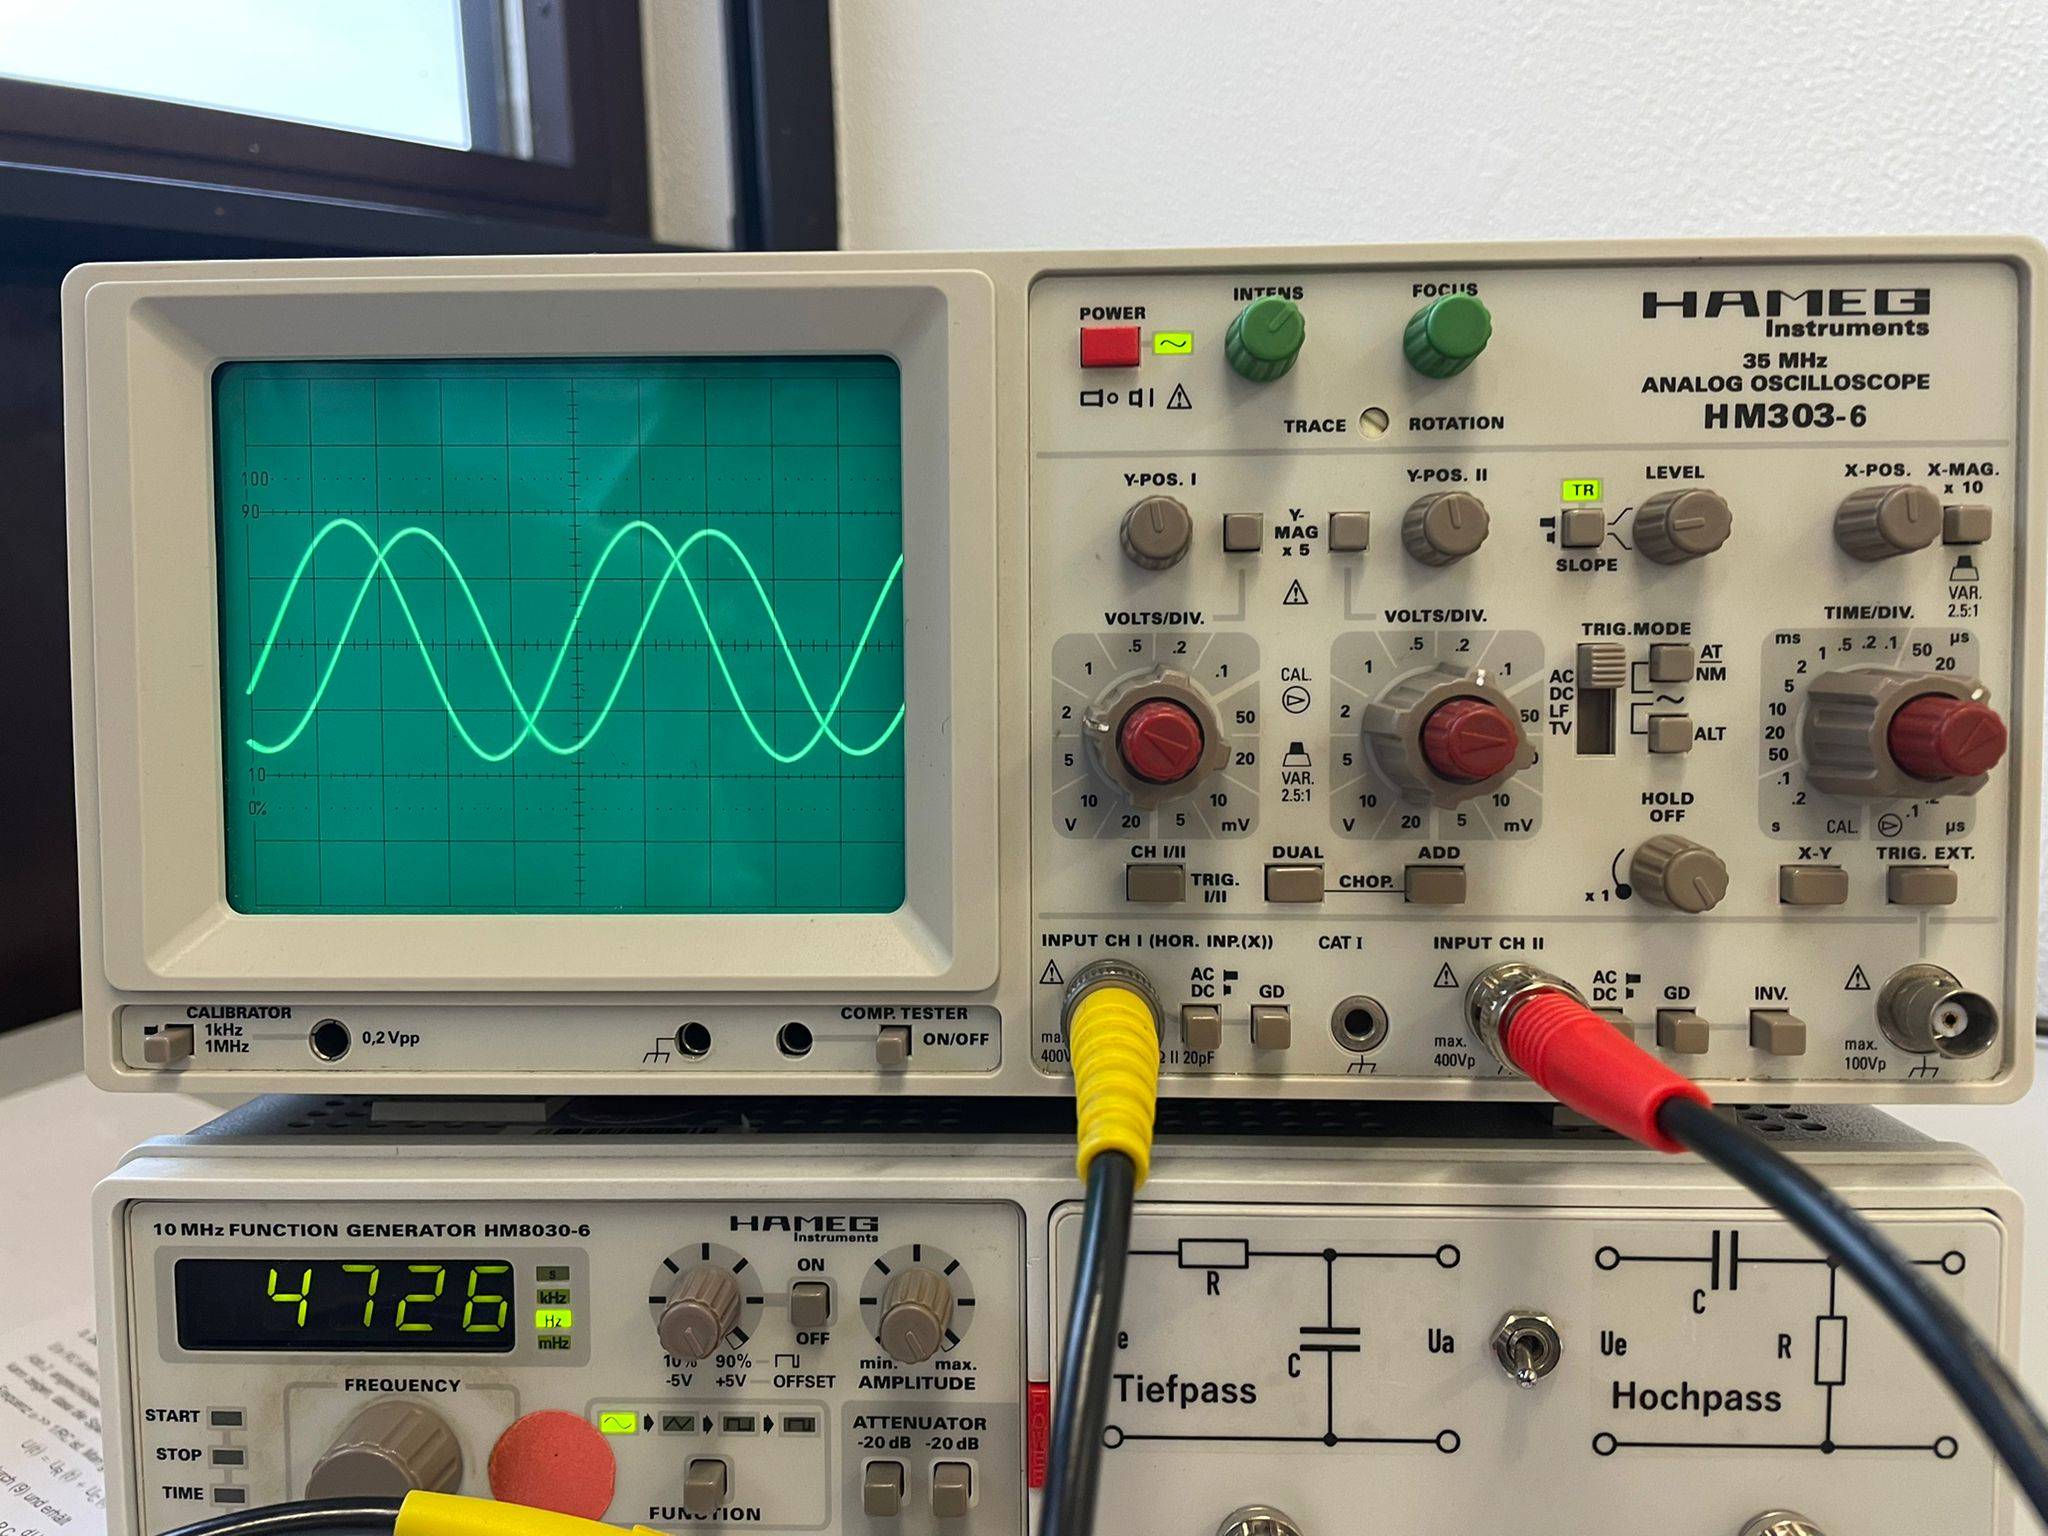
\includegraphics[scale=0.1]{content/sinInt.png}
    \caption{sin}
  \end{subfigure}
  \hfill
  \begin{subfigure}{0.48\textwidth}
    \centering
    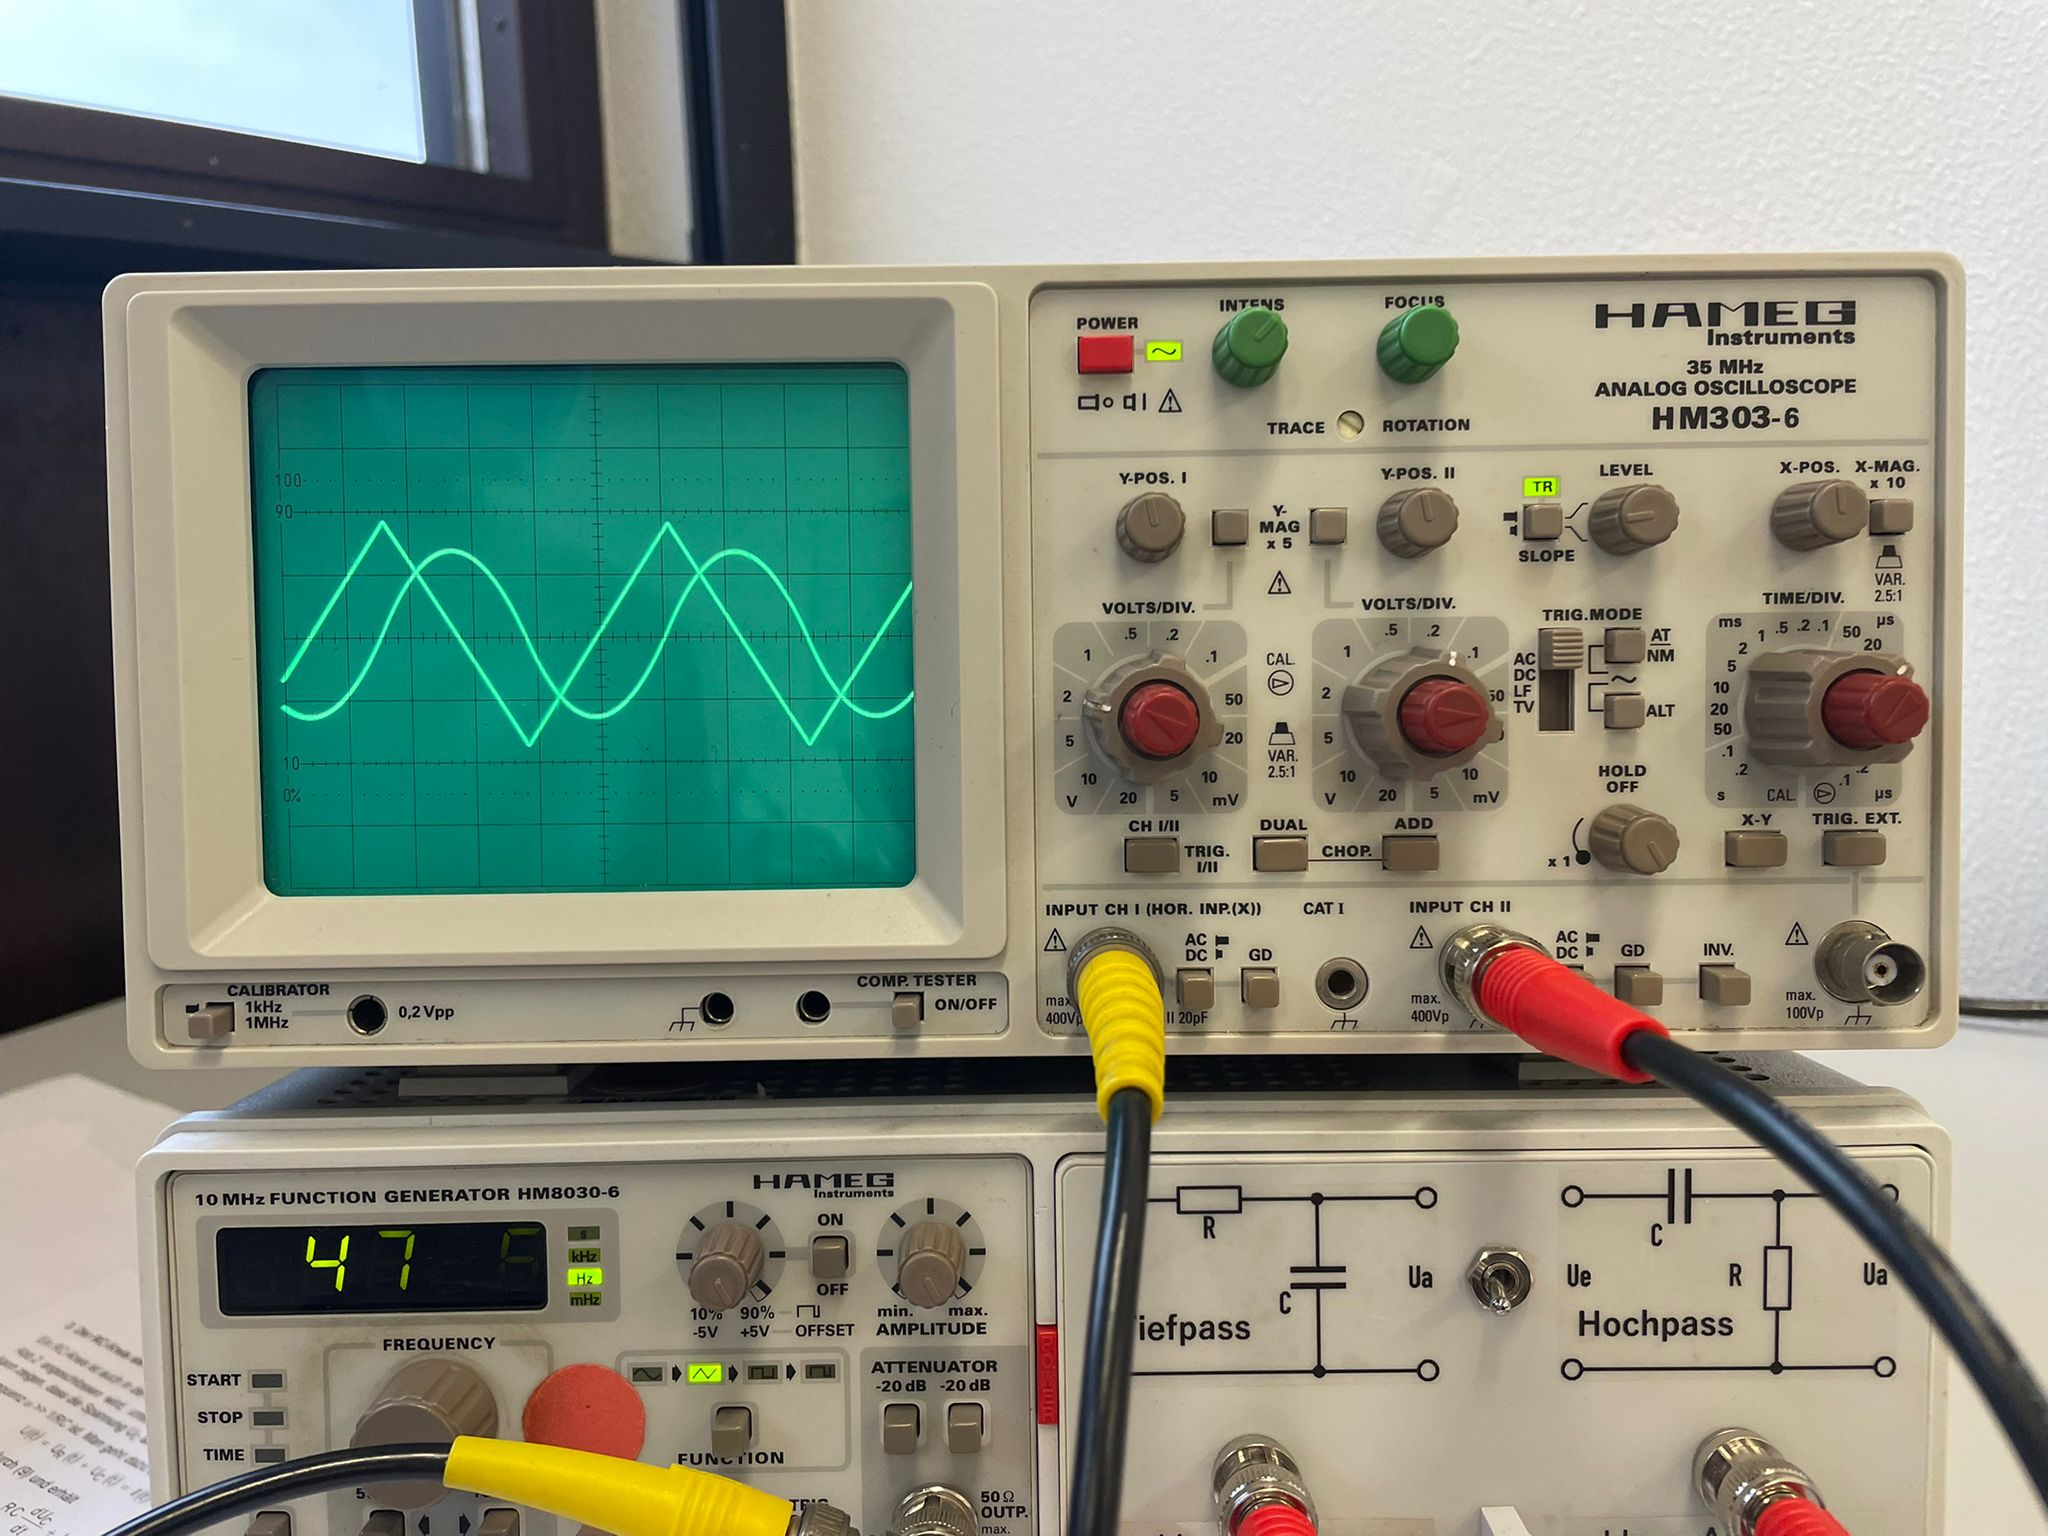
\includegraphics[scale=0.1]{content/saegInt.png}
    \caption{Sägezahn}
  \end{subfigure}
  \caption{}
  \label{fig:abb9}
\end{figure}

\begin{figure}
  
  \centering
  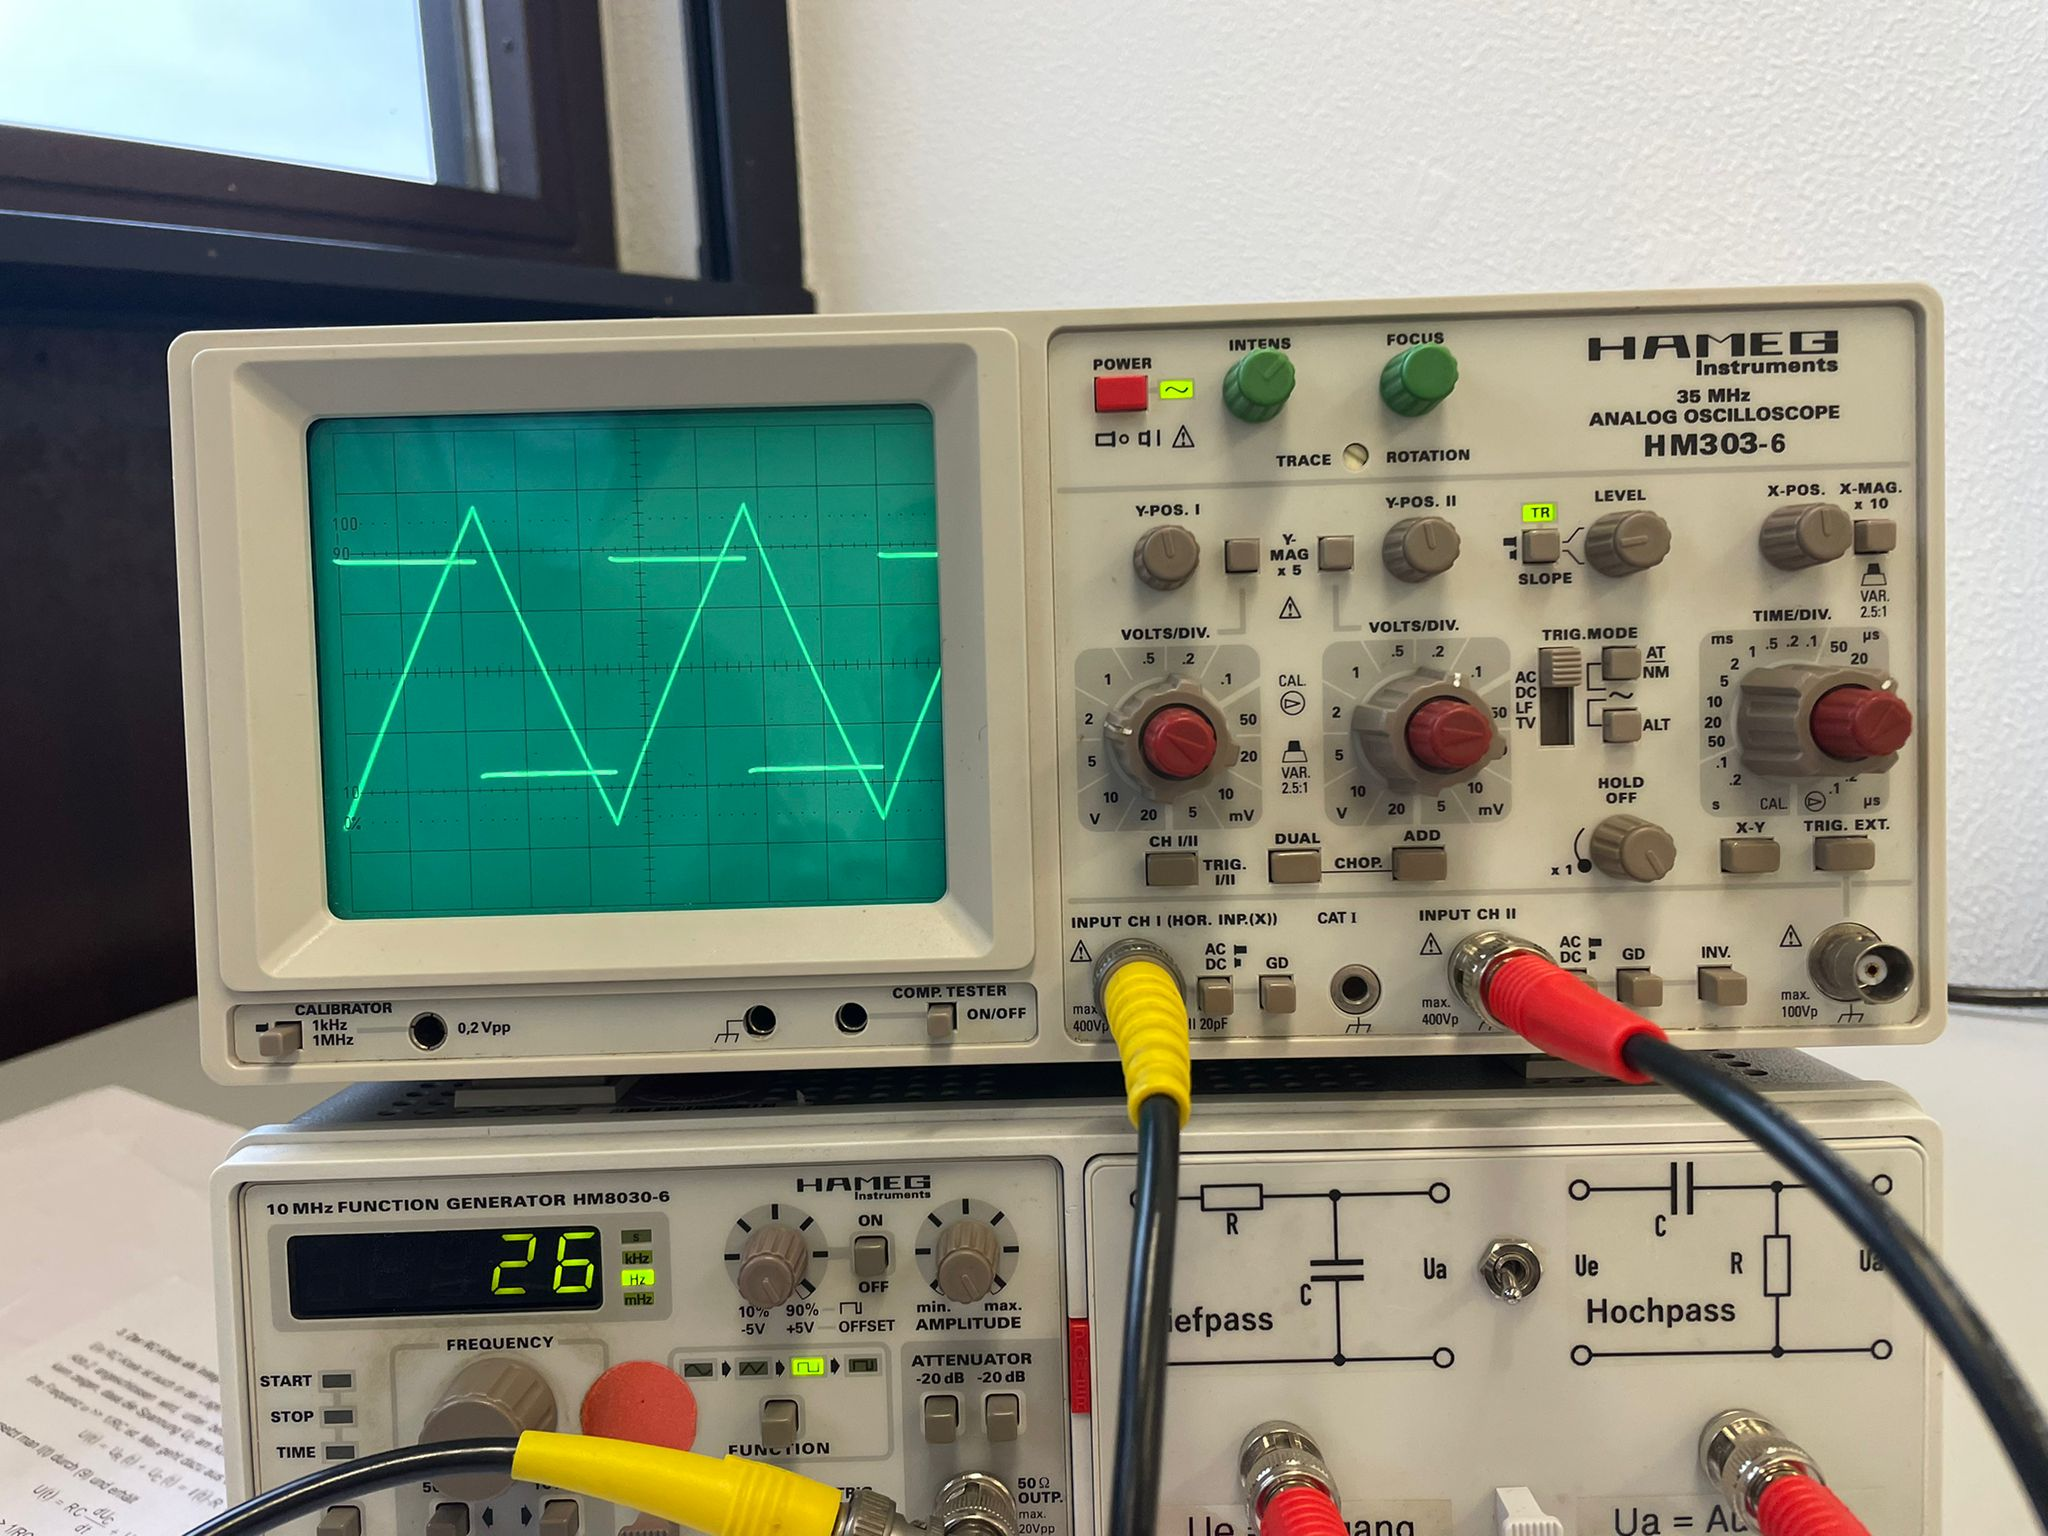
\includegraphics[scale=0.1]{content/rechteckInt.png}
  \caption{Rechteck}
  \label{fig:abb10}
\end{figure}
